
  \documentclass{exam}

  \usepackage{units} 
  \usepackage{graphicx}
  \usepackage[fleqn]{amsmath}
  \usepackage{cancel}
  \usepackage{float}
  \usepackage{mdwlist}
  \usepackage{booktabs}
  \usepackage{cancel}
  \usepackage{polynom}
  \usepackage{caption}
  \usepackage{fullpage}
  \usepackage{xfrac}
  \usepackage{enumerate}

  \newcommand{\degree}{\ensuremath{^\circ}} 
  \everymath{\displaystyle}

  % \begin{figure}[H]
  %   \centering
  %   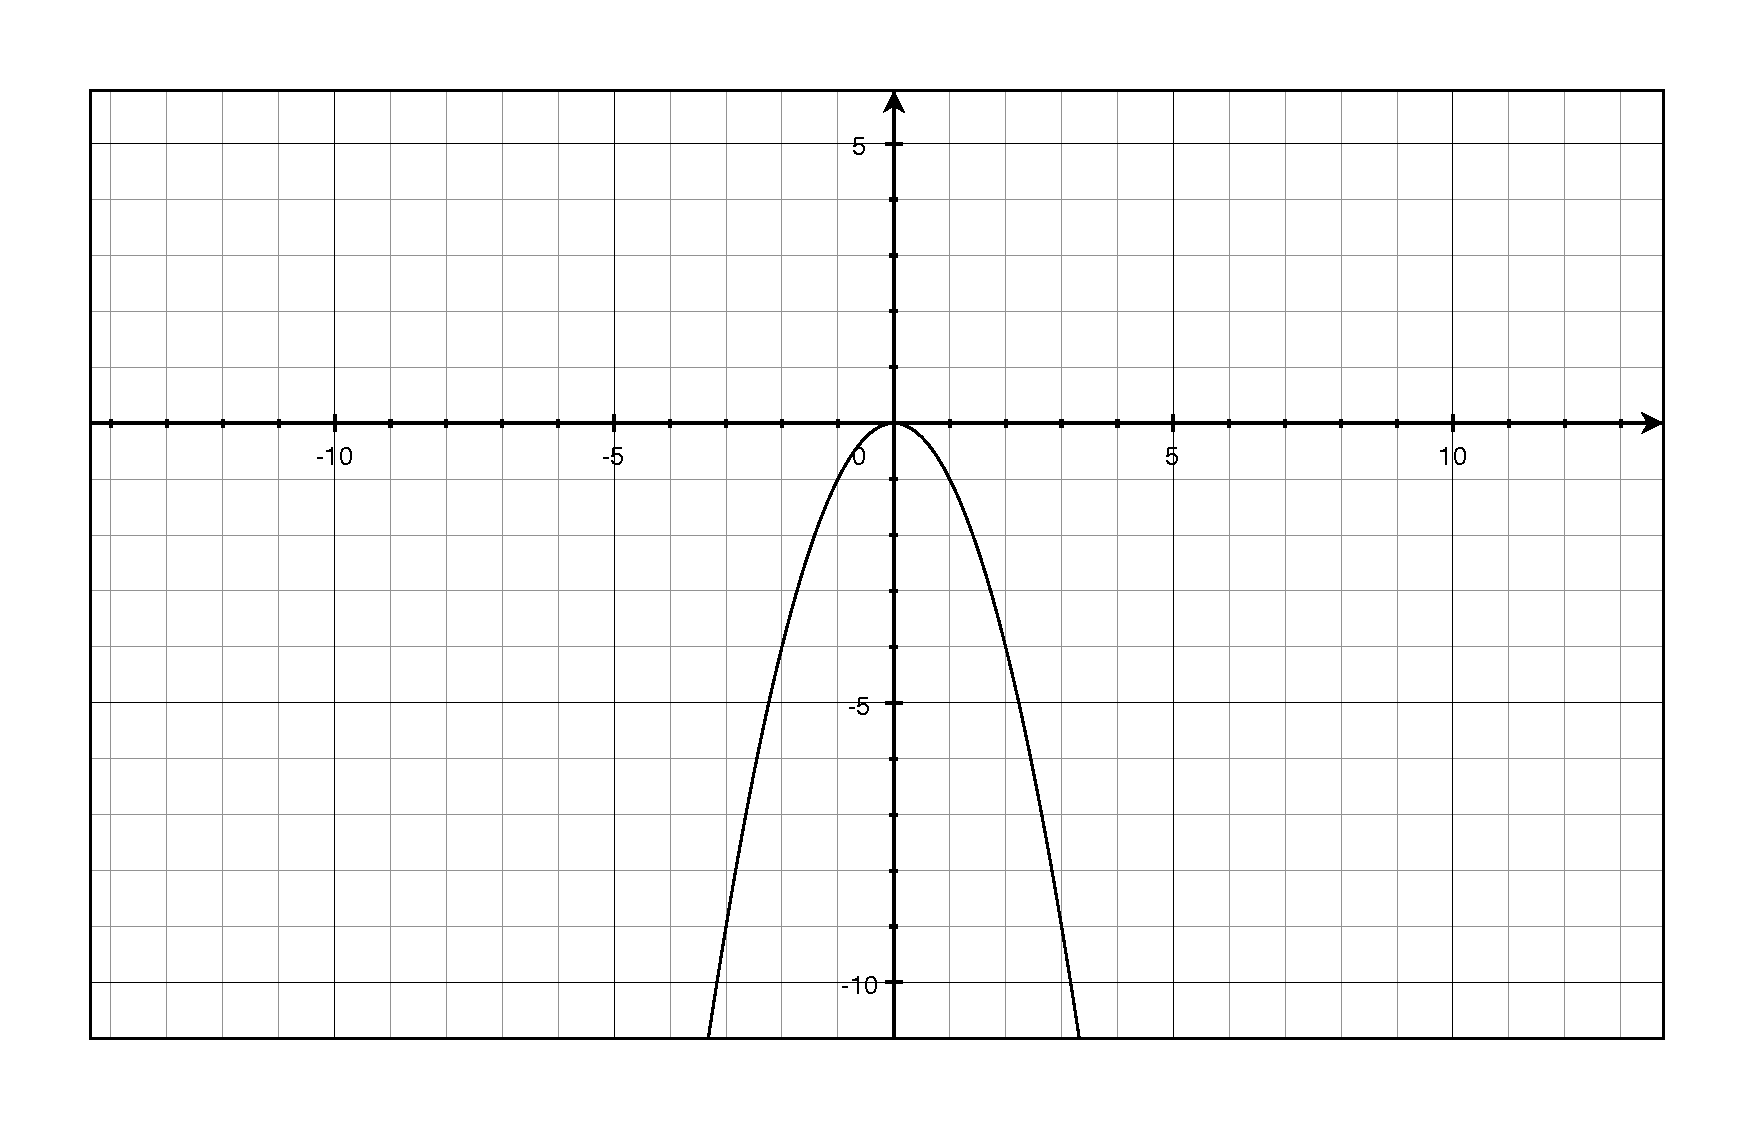
\includegraphics[scale=0.8]{problem7.eps}
  %   \caption*{Problem 7}
  % \end{figure}

  % \begin{tabular}{cc}
  %   \toprule
  %   period & amplitude \\
  %   \midrule
  %   value one & value two
  %   \bottomrule
  % \end{tabular}

  \printanswers

  \ifprintanswers 
    \usepackage{2in1, lscape} 
  \fi

  \date{June 26, 2013}
  \author{}
  \title{Math 141 \\ Homework 16}

  \begin{document}

    \maketitle

    \section{Homework}

    Section 4.4: 7-24, 27-34, 41-51, 67-77, 81

    \ifprintanswers
      \pagebreak
    \fi

    \section{Extra Credit}
    Section 4.4: 52-54

    \ifprintanswers
      \begin{description}
        \item[52] 
          \begin{align*}
            (\log x)^3                &= 3 \log x \\
            (\log x)^3 - 3 \log x     &= 0 \\
            \log x \left[(\log x)^2 - 3 \right] &= 0 \\
            \\
            \log x &= 0 \\
            x      &= 1 \\
            \\
            (\log x)^2 - 3 &= 0 \\
            (\log x)^2     &= 3 \\
            \log x         &= \pm \sqrt{3} \\
            x              &= 10^{\pm \sqrt{3}} \\
            \\
            x &= \boxed{\left\{ 1, 10^{\sqrt{3}}, 10^{ - \sqrt{3}} \right\} } \\
          \end{align*}
          
        \item[53] 
          \begin{align*}
            2^{2/\log_5 x}        &= \frac{1}{16} \\
            \log_2 2^{2/\log_5 x} &= \log_2 \frac{1}{16} \\
            2/\log_5 x            &= - 4 \\
            \log_5x               &= - \frac{1}{2} \\
            x                     &= \boxed{\frac{1}{\sqrt{5}}} \\
          \end{align*}

        \item[54] 
          \begin{align*}
            \log_2 (\log_3 x) &= 4 \\
            \log_3 x          &= 2^4 \\
            \log_3 x          &= 16 \\
            x                 &= \boxed{3^{16}} \\
          \end{align*}

      \end{description}
    \fi

    \section{Review}

    Find all the real zeros
    \begin{enumerate}
      \item $2x^3 + 5x^2 - 23x + 10 = 0$
        \ifprintanswers
          $x = \left\{ 2, -5, \frac{1}{2} \right\}$
        \fi

      \item $x^4 + 2x^3 - 9x^2 - 18x = 0$
        \ifprintanswers
          $x = \left\{ 3, -3, 2 \right\}$
        \fi
    \end{enumerate}

  \ifprintanswers
    \section{Section 4.4}

    \begin{description}

      \item[7]
        \begin{align*}
          3 e^x &= 10 \\
          e^x   &= \frac{10}{3} \\
          x     &= \ln \frac{10}{3} \\
                &\approx \boxed{1.20397} \\
        \end{align*}

      \item[8]
        \begin{align*}
          4 e^{12x} &= 17 \\
          e^{12x}   &= \frac{17}{4} \\
          x         &= \frac{1}{12} \ln \frac{17}{4} \\
                    &\approx \boxed{0.120577} \\
        \end{align*}

      \item[9]
        \begin{align*}
          e^{1 - 4x} &= 2 \\
          1 - 4x     &= \ln 2 \\
          4x         &= 1 - \ln 2 \\
          x          &= \frac{1 - \ln 2}{4} \\
                     &\approx \boxed{0.0767132} \\
        \end{align*}

      \item[10]
        \begin{align*}
          4 (1 + 10^{5x}) &= 9 \\
          1 + 10^{5x}     &= \frac{9}{4} \\
          10^{5x}         &= \frac{5}{4}\\
          x               &= \frac{1}{5} \log \frac{5}{4} \\
                          &\approx \boxed{0.019382} \\
        \end{align*}

      \item[11]
        \begin{align*}
          4 + 3^{5x} &= 8 \\
          3^{5x}     &= 4 \\
          5x         &= \log_3 4 \\
          x          &= \frac{1}{5} \log_3 4 \\
                     &\approx \boxed{0.252372} \\
        \end{align*}

      \item[12]
        \begin{align*}
          2^{3x} &= 34 \\
          3x     &= \log_2 34 \\
          x      &= \frac{1}{3} \log_2 34 \\
                 &\approx \boxed{1.69582} \\
        \end{align*}

      \item[13]
        \begin{align*}
          8^{0.4x} &= 5 \\
          0.4x &= \log_8 5 \\
          x    &= \frac{\log_8 5}{0.4} \\
               &\approx \boxed{1.93494} \\
        \end{align*}

      \item[14]
        \begin{align*}
          3^{x/14}     &= 0.1 \\
          \frac{x}{14} &= \log_3 0.1 \\
          x            &= 14 \log_3 0.1 \\
                       &\approx \boxed{-29.3426} \\
        \end{align*}

      \item[15]
        \begin{align*}
          5^{-x/100}     &= 2 \\
          -\frac{x}{100} &= \log_5 2 \\
          x              &= -100 \log_5 2 \\
                         &\approx \boxed{-43.0677} \\
        \end{align*}

      \item[16]
        \begin{align*}
          e^{3 - 5x} &= 16 \\
          3 - 5x     &= \ln 16 \\
          5x         &= 3 - \ln 16 \\
          x          &= \frac{3 - \ln 16}{5} \\
                     &\approx \boxed{0.0454823} \\
        \end{align*}

      \item[17]
        \begin{align*}
          e^{2x + 1} &= 200 \\
          2x + 1     &= \ln 200 \\
          2x         &= \ln 200 - 1 \\
          x          &= \frac{\ln 200 - 1}{2} \\
                     &\approx \boxed{2.14916} \\
        \end{align*}

      \item[18]
        \begin{align*}
          \left( \frac{1}{4} \right)^x &= 75 \\
          4^{-x}                       &= 75 \\
          x                            &= -\log_4 75 \\
                                       &\approx \boxed{-3.11441} \\
        \end{align*}

      \item[19]
        \begin{align*}
          5^x               &= 4^{x + 1} \\
          \ln 5^x           &= \ln 4^{x + 1} \\
          x \ln 5           &= (x  + 1) \ln 4 \\
          x \ln 5           &= x \ln 4 + \ln 4 \\
          x \ln 5 - x \ln 4 &= \ln 4 \\
          x                 &= \frac{\ln 4}{\ln 5 - \ln 4} \\
                            &\approx \boxed{6.21257} \\
        \end{align*}

      \item[20]
        \begin{align*}
          10^{1 - x}         &= 6^x \\
          \ln 10^{1 - x}     &= \ln 6^x \\
          (1 - x) \ln 10     &= x \ln 6 \\
          \ln 10 - x \ln 10  &= x \ln 6 \\
          x \ln 6 + x \ln 10 &= \ln 10 \\
          x                  &= \frac{\ln 10}{\ln 6 + \ln 10} \\
                             &\approx \boxed{0.562382} \\
        \end{align*}

      \item[21]
        \begin{align*}
          2^{3x + 1}          &= 3^{x - 2} \\
          (3x + 1) \ln 2      &= (x - 2) \ln 3 \\
          x (3 \ln 2 - \ln 3) &= - 2 \ln 3 - \ln 2 \\
          x                   &= \frac{ - 2 \ln 3 - \ln 2}{3 \ln 2 - \ln 3} \\
                              &\approx \boxed{-2.94687} \\
        \end{align*}

      \item[22]
        \begin{align*}
          7^{x/2}             &= 5^{1 - x} \\
          \frac{x \ln 7}{2}   &= (1 - x) \ln 5 \\
          x \ln 7             &= (2 - 2x) \ln 5 \\
          x (\ln 7 + 2 \ln 5) &= 2 \ln 5 \\
          x                   &= \frac{2 \ln 5}{\ln 7 + 2 \ln 5} \\
                              &\approx \boxed{0.623235} \\
        \end{align*}

      \item[23]
        \begin{align*}
          \frac{50}{1 + e^x} &= 4 \\
          50                 &= 4 + 4e^x \\
          4e^x               &= 46 \\
          x                  &= \ln \frac{23}{2} \\
                             &\approx \boxed{2.44235} \\
        \end{align*}

      \item[24]
        \begin{align*}
          \frac{10}{1 + e^{-x}} &= 2 \\
          10                    &= 2 + 2e^{-x} \\
          5                     &= 1 + e^{-x} \\
          e^{-x}                &= 4 \\
          x                     &= -\ln 4 \\
                                &\approx \boxed{-1.38629} \\
        \end{align*}

      \item[27]
        \begin{align*}
          x^2 2^x - 2^x              &= 0 \\
          2^x \left( x^2 - 1 \right) &= 0 \\
          2^x(x + 1)(x - 1)          &= 0 \\
          x                          &= \boxed{ \{ -1, 1 \} } \\
        \end{align*}

      \item[28]
        \begin{align*}
          x^2 10^x - x 10^x           &= 2(10^x) \\
          x^2 10^x - x 10^x - 2(10^x) &= 0 \\
           10^x (x^2  - x  - 2)       &= 0 \\
           10^x (x - 2)(x + 1)        &= 0 \\
          x                           &= \boxed{ \{ -1, 2 \} } \\
        \end{align*}

      \item[31]
        \begin{align*}
          e^{2x} - 3e^x + 2  &= 0 \\
          (e^x - 2)(e^x - 1) &= 0 \\
          x                  &= \boxed{ \{ 0, \ln 2 \} } \\
        \end{align*}

      \item[35] 
        \begin{align*}
          \ln x &= 10 \\
          x     &= \boxed{e^{10}} \\
        \end{align*}

      \item[36] 
        \begin{align*}
          ln (2 + x) &= 1 \\
          2 + x      &= e \\
          x          &= \boxed{e - 2} \\
        \end{align*}

      \item[37] 
        \begin{align*}
          \log x &= -2 \\
          x      &= 10^{-2} \\
                 &= \boxed{\frac{1}{100}} \\
        \end{align*}

      item[38] 
        \begin{align*}
          \log (x - 4) &= 3 \\
          x - 4        &= 10^3 \\
          x            &= \boxed{996} \\
        \end{align*}

      \item[39] 
        \begin{align*}
          \log (3x + 5) &= 2 \\
          3x + 5        &= 10^2 \\
          x             &= \boxed{\frac{95}{3}} \\
        \end{align*}

      \item[40] 
        \begin{align*}
          \log_2 (2 - x) &= 3 \\
          2 - x          &= 2^3 \\
          x              &= \boxed{-6} \\
        \end{align*}

      \item[41] 
        \begin{align*}
          2 - \ln(3 - x) &= 0 \\
          \ln(3 - x)     &= 2 \\
          3 - x          &= e^2 \\
          x              &= \boxed{3 - e^2} \\
        \end{align*}

      \item[42] 
        \begin{align*}
          \log_2(x^2 - x - 2) &= 2 \\
          x^2 - x - 2         &= 2^2 \\
          x^2 - x - 6         &= 0 \\
          (x - 3)(x + 2)      &= 0 \\
          x                   &= \boxed{\{ - 2, 3\}} \\
        \end{align*}

      \item[43] 
        \begin{align*}
          \log_2 3 + \log_2 x &= \log_2 5 + \log_2(x - 2) \\
          \log_2 3x           &= \log_2 [5 (x - 2)] \\
          3x                  &= 5x - 10 \\
          x                   &= \boxed{5} \\
        \end{align*}

      \item[44] 
        \begin{align*}
          2 \log x       &= \log 2 + \log(3x - 4) \\
          \log x^2       &= \log [2(3x - 4)] \\
          x^2            &= 6x - 8 \\
          x^2 - 6x + 8   &= 0 \\
          (x - 4)(x - 2) &= 0 \\
          x              &= \boxed{\{2, 4\}} \\
        \end{align*}

      \item[45] 
        \begin{align*}
          \log x + \log(x - 1) &= \log (4x) \\
          \log [x(x - 1)]      &= \log (4x) \\
          x^2 - x              &= 4x \\
          x^2 - 5x             &= 0 \\
          x(x - 5)             &= 0 \\
          x                    &= \boxed{5} \\
        \end{align*}

      \item[46] 
        \begin{align*}
          \log_5 x + \log_5(x + 1) &= \log_5 20 \\
          \log_5 [x(x + 1)]        &= \log_5 20 \\
          x^2 + x                  &= 20 \\
          x^2 + x - 20             &= 0 \\
          (x + 5)(x - 4)           &= 0 \\
          x                        &= \boxed{4} \\
        \end{align*}

      \item[47] 
        \begin{align*}
          \log_5 (x + 1) - \log_5 (x - 1) &= 2 \\
          \log_5 \frac{x + 1}{x - 1}      &= 2 \\
          \frac{x + 1}{x - 1}             &= 5^2 \\
          x + 1                           &= 25x - 25 \\
          24x                             &= 26 \\
          x                               &= \boxed{\frac{13}{12}} \\
        \end{align*}

      \item[48] 
        \begin{align*}
          \log x + \log (x - 3)        &= 1 \\
          \log \left( x^2 - 3x \right) &= 1 \\
          x^2 - 3x                     &= 10 \\
          x^2 - 3x - 10                &= 0 \\
          (x - 5)(x + 2)               &= 0 \\
          x                            &= \boxed{5} \\
        \end{align*}

      \item[51] 
        \begin{align*}
          \log (x + 3) &= \log x + \log 3 \\
          \log (x + 3) &= \log (3x) \\
           x + 3       &= 3x \\
           2x          &= 3 \\
           x           &= \boxed{\frac{3}{2}} \\
        \end{align*}

      \item[67]
        $A(t) = 5000 e^{0.085 t}$

        \begin{enumerate}[a]
          \item $A(3) = 5000 e^{0.085 \cdot 3} = \boxed{\$6,452.31}$

          \item
            \begin{align*}
              10000 &= 5000 e^{0.085 t} \\
              2     &= e^{0.085 t} \\
              \ln 2 &= 0.085t \\
              t     &= \boxed{\unit[8.15]{year}} \\
            \end{align*}
        \end{enumerate}

      \item[68]
        $A(t) = 6500 e^{0.06 t}$

        \begin{enumerate}[a]
          \item $A(2) = 6500 e^{0.06 t} = \boxed{\$7,328.73}$

          \item
            \begin{align*}
              8000 &= 6500 e^{0.06 t} \\
              t     &= \boxed{\unit[3.46]{year}} \\
            \end{align*}
        \end{enumerate}

      \item[69]
        \begin{align*}
          8000    &= 5000 \left( 1 + \frac{0.075}{4} \right)^{4t} \\
          % 1.6     &= (1.01875)^{4t} \\
          % \ln 1.6 &= 4t \ln 1.01875 \\
          t       &= \frac{\ln 1.6}{4 \ln 1.01875} \\
                  &\approx \boxed{\unit[6.33]{years}} \\
        \end{align*}

      \item[75]
        \begin{align*}
          5 &= 15 e^{-0.087t} \\
          t &= \frac{\ln 1/3}{-0.087} \\
            &\approx \boxed{\unit[12.63]{days}} \\
        \end{align*}

      \item[76]
        \begin{align*}
          70          &= 80 \left( 1 - e^{-0.2t} \right) \\
          % \frac{1}{8} &= e^{-0.2t} \\
          t           &= \frac{\ln 1/8}{-0.2} \\
                      &\approx \boxed{\unit[10.4]{seconds}} \\
        \end{align*}

      \item[77]
        \begin{enumerate}[a]
          \item $P(3) = \frac{10}{1 + 4e^{-0.8 \cdot 3}} = \unit[7,337]{fish}$

          \item 
            \begin{align*}
              5 &= \frac{10}{1 + 4e^{-0.8t}} \\
              % 2 &= 1 + 4e^{-0.8t} \\
              t &= \frac{\ln 0.25}{-0.8} \\
                &\approx \boxed{\unit[1.73]{years}} \\
            \end{align*}
        \end{enumerate}

      \item[81]
        \begin{enumerate}[a]
          \item 
            \begin{align*}
              I &= \frac{60}{13}\left( 1 - e^{-13t/5} \right) \\
              1 - \frac{60 I}{14} &= e^{-13t/5} \\
            \end{align*}

        \end{enumerate}

    \end{description}

  \else
    \vspace{6 cm}
    \begin{quote}
      \begin{em}
        States are violent institutions. The government of any country, including ours, represents some sort of domestic
        power structure, and it's usually violent. States are violent to the extent that they're powerful, that's
        roughly accurate.

        % The political policies that are called conservative these days would appall any genuine conservative, if
        % there were one around to be appalled. For example, the central policy of the Reagan Administration - which
        % was supposed to be conservative - was to build up a powerful state. The state grew in power more under
        % Reagan than in any peacetime period, even if you just measure it by state expenditures. The state
        % intervention in the economy vastly increased. That's what the Pentagon system is, in fact; it's the creation
        % of a state-guaranteed market and subsidy system for high-technology production.

        % The ``corporatization of America'' during the past century has been an attack on democracy—and on markets,
        % part of the shift from something resembling "capitalism" to the highly administered markets of the modern
        % state/corporate era. A current variant is called "minimizing the state," that is, transferring decision-making
        % power from the public arena to somewhere else: "to the people" in the rhetoric of power; to private tyrannies,
        % in the real world.
      \end{em}
    \end{quote}
    \hspace{1 cm} --Noam Chomsky 
  \fi


\end{document}

